
%(BEGIN_QUESTION)
% Copyright 2009, Tony R. Kuphaldt, released under the Creative Commons Attribution License (v 1.0)
% This means you may do almost anything with this work of mine, so long as you give me proper credit

Here is an oscilloscope's view of an eight-bit data stream sent asynchronously with no parity bit, using {\it NRZ} (Non-Return to Zero) encoding:

$$\includegraphics[width=15.5cm]{i02368x01.eps}$$

Identify the binary data represented by this waveform, and express it in hexadecimal form as well.

\vskip 20pt \vbox{\hrule \hbox{\strut \vrule{} {\bf Suggestions for Socratic discussion} \vrule} \hrule}

\begin{itemize}
\item{} Explain why it is critically important that we know in advance this is an {\it eight-bit} data frame.
\item{} In this particular example, is the number of stop bits significant?  Why or why not?
\end{itemize}

\underbar{file i02368}
%(END_QUESTION)





%(BEGIN_ANSWER)

\noindent
{\bf Partial answer:}

Hex = 7C

%(END_ANSWER)





%(BEGIN_NOTES)

$$\includegraphics[width=15.5cm]{i02368x02.eps}$$

The trick to decoding data here is knowing there are {\it eight} data bits, and figuring out how wide each one is.

%INDEX% Networking, serial data: asynchronous data format
%INDEX% Networking, serial data: start bit
%INDEX% Networking, serial data: stop bit

%(END_NOTES)


